\documentclass[10pt,a4paper]{article}
\usepackage[margin=21mm,headheight=15pt]{geometry}
\usepackage[T1]{fontenc}
\usepackage{lmodern,amsmath,amssymb,tikz,graphicx,hyperref,fancyhdr,enumitem}
\usetikzlibrary{arrows.meta,positioning,calc,decorations.pathmorphing}
\definecolor{ink}{RGB}{20,53,78}
\hypersetup{colorlinks=true,urlcolor=ink,linkcolor=ink}
\setlength{\parindent}{0pt}\setlength{\parskip}{5pt}
\emergencystretch=3em
\pagestyle{fancy}\fancyhf{}\fancyfoot[C]{\thepage}
\renewcommand{\headrulewidth}{.3pt}
\newcommand{\task}[2]{\par\medskip{\color{ink}\Large\bfseries #1. #2}\par\smallskip}
\newcommand{\answer}{\par\smallskip\textbf{Worked reasoning.} }
\setlist[enumerate]{label=\textbf{(\alph*)},leftmargin=7mm,itemsep=7pt}
\begin{document}
\fancyhead[L]{\small Control of Dynamical Systems}
\fancyhead[R]{\small Laboratory 07}
{\color{ink}\LARGE\bfseries Laboratory 07}\par
{\large A feedback loop with a communication delay}\par
\textbf{Worked solutions -- five integrated problems}\par
{\small\textbf{Evidence boundary.} Original hypothetical scenarios. Derive, calculate and justify decisions; every numerical record is synthetic. Figures are conceptual and not to scale.}
\smallskip\textbf{Shared nominal data.} Nominal loop: $L(s)=8e^{-Ts}/[s(s+3)]$, unity negative feedback, and ideal constant delay $T$. Exact-delay results and rational Pad\'e approximations must be distinguished.
\task{1}{A remotely observed actuator}
A sensor observes a moving carriage through a communication link. Use the declared delay-free loop and distinguish its physical dynamics from the additional time spent transporting information.
\begin{center}\resizebox{\ifdim\width>.98\linewidth.98\linewidth\else\width\fi}{!}{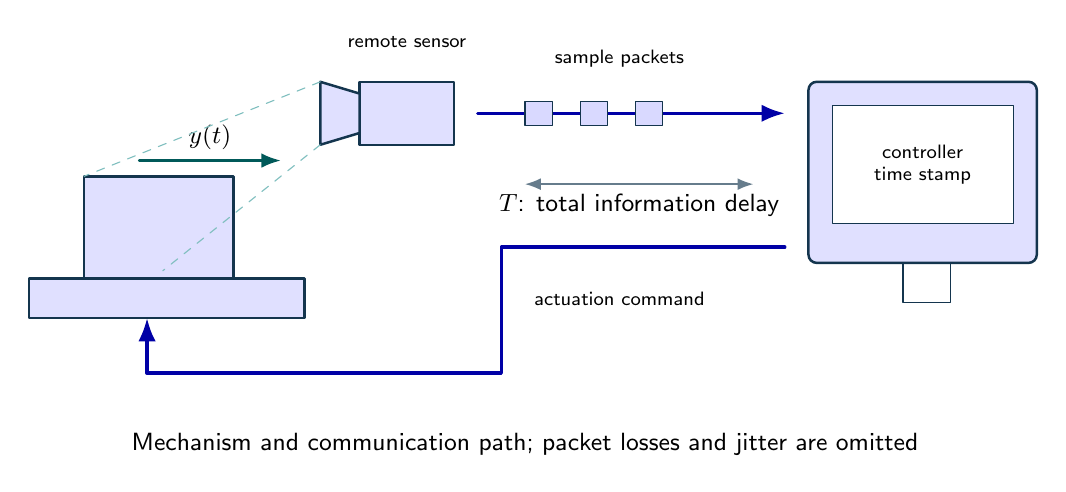
\begin{tikzpicture}[
font=\sffamily\small,>=Latex,line cap=round,line join=round,
wall/.style={draw=ink,line width=1.2pt,fill=blue!5},
water/.style={fill=cyan!25,draw=none},
metal/.style={draw=ink,fill=blue!12,line width=.9pt},
flow/.style={->,draw=blue!65!black,line width=1.2pt},
heat/.style={->,draw=orange!85!black,line width=1.1pt},
measure/.style={->,draw=teal!70!black,line width=.9pt},
dim/.style={<->,draw=ink!65,line width=.6pt},
spring/.style={draw=ink,decorate,decoration={coil,aspect=.5,segment length=4pt,amplitude=3pt}},
wire/.style={draw=ink,line width=1pt},
lab/.style={align=center,font=\sffamily\small},
smalllab/.style={align=center,font=\sffamily\scriptsize}]

\draw[metal](.5,1)rectangle(4,1.5);
\draw[metal](1.2,1.5)rectangle(3.1,2.8);
\draw[measure](1.9,3)--(3.7,3)node[midway,above]{$y(t)$};
\draw[metal](4.7,3.2)rectangle(5.9,4);
\draw[metal](4.7,3.35)--(4.2,3.2)--(4.2,4)--(4.7,3.85)--cycle;
\draw[teal!50,dashed](4.2,3.2)--(2.2,1.6)(4.2,4)--(1.2,2.8);
\node[smalllab]at(5.3,4.5){remote sensor};
\draw[metal,rounded corners=3pt](10.4,1.7)rectangle(13.3,4);
\draw[fill=white,draw=ink](10.7,2.2)rectangle(13,3.7);
\draw[ink](11.6,1.7)--(11.6,1.2)--(12.2,1.2)--(12.2,1.7);
\node[smalllab]at(11.85,2.95){controller\\time stamp};
\draw[flow](6.2,3.6)--(10.1,3.6);
\foreach \x in {6.8,7.5,8.2}{\draw[fill=blue!15,draw=ink](\x,3.45)rectangle++(.35,.3);}
\node[smalllab]at(8,4.3){sample packets};
\draw[flow](10.1,1.9)--(6.5,1.9)--(6.5,.3)--(2,.3)--(2,1);
\node[smalllab]at(8,1.25){actuation command};
\draw[dim](6.8,2.7)--node[below]{$T$: total information delay}(9.7,2.7);
\node[lab]at(6.8,-.6){Mechanism and communication path; packet losses and jitter are omitted};
\end{tikzpicture}
}\par{\small A remote mechanism sends measurements and receives commands through a communication path. The model combines those latencies into one ideal constant delay; the drawn packet train is not an experimental record.}\end{center}
\begin{enumerate}
\item The loop is $L_0(s)=8/[s(s+3)]$ with unity negative feedback. Derive its closed-loop poles, natural frequency and damping ratio.
\answer The characteristic equation is $s^2+3s+8=0$. Its roots are $(-3\pm j\sqrt{23})/2$, with negative real parts. Matching $s^2+2\zeta\omega_n s+\omega_n^2$ gives $\omega_n=\sqrt8$ and $\zeta=3/(2\sqrt8)\approx0.53033$. This establishes nominal delay-free stability before interpreting a phase margin or added-delay limit.
\item Find the unique positive gain crossover of $L_0$. Show why an ideal pure delay $e^{-sT}$ does not change this crossover.
\answer Magnitude satisfies $|L_0(j\omega)|=8/[\omega\sqrt{\omega^2+9}]$. Setting it to one and writing $z=\omega^2$ gives $z^2+9z-64=0$. Thus $\omega_c=\sqrt{(-9+\sqrt{337})/2}$. The other quadratic root is negative and does not give a real positive frequency. Since $|e^{-j\omega T}|=1$, a pure delay leaves the magnitude equation and its crossover unchanged.
\item Write the exact delayed closed-loop characteristic equation. Explain why the delay-free second-order poles or any finite-order approximation do not list all modes of the delayed system.
\answer Unity negative feedback gives $1+8e^{-sT}/[s(s+3)]=0$, or $s(s+3)+8e^{-sT}=0$. For $T>0$ this is transcendental, not a second-order polynomial, and generally has infinitely many roots. The delay-free pair describes only the $T=0$ case. A finite Padé model supplies a finite set of approximate modes, so its conclusions must be checked against the exact delay model or a justified delay-margin calculation.
\end{enumerate}

\newpage
\task{2}{Allocating a finite phase budget}
The loop must retain a stated phase margin after communication, computation and actuation delays. Budget the total delay rather than considering each component separately.
\begin{enumerate}
\item Calculate the nominal phase margin and the first positive pure-delay boundary. Express the formulas exactly before giving approximate values.
\answer For positive frequency, the loop phase is $-\pi/2-\arctan(\omega/3)$. The margin is $\phi_m=\pi/2-\arctan(\omega_c/3)\approx54.208^\circ$. Delay adds phase $-\omega_cT$, so the first boundary is $T_{crit}=\phi_m/\omega_c\approx0.4374$ s. The delay-free loop is stable and has a unique positive magnitude crossing. These facts justify identifying this first phase crossing as the initial loss of stability for this loop.
\item Find the maximum constant delay that retains at least a 30 degree phase margin. Compare it with delays of 0.1 s and 0.3 s.
\answer At crossover the remaining margin is $\phi_m-\omega_cT$. Therefore $T\le(\phi_m-\pi/6)/\omega_c\approx0.1953$ s. A 0.1 s delay leaves about $41.814^\circ$ and meets the requirement. A 0.3 s delay leaves about $17.028^\circ$ and fails it, although it is still below the first stability boundary. A performance margin requirement can be stricter than mere nominal stability.
\item Assume constant pure delays of 0.12 s, 0.04 s, 0.02 s and 0.01 s in successive stages. Determine whether their combined delay satisfies the 30-degree requirement and calculate the remaining unused delay allowance.
\answer Pure delays in series add, giving $T_{\rm total}=0.19$ s. The 30-degree allowance is $(PM_0-\pi/6)/\omega_c\simeq0.195329$ s, so the remaining allowance is about 0.005329 s. The retained phase margin is $PM_0-0.19\omega_c$ radians, slightly above 30 degrees. This result assumes constant pure delays and the same single crossover; omitted lag dynamics or arbitrary jitter are different models.
\end{enumerate}

\newpage
\task{3}{How a low-order delay approximation can overstate tolerance}
Compare the exact phase contribution with a first-order rational approximation. Use the comparison to audit a claimed stability boundary.
\begin{center}\resizebox{\ifdim\width>.98\linewidth.98\linewidth\else\width\fi}{!}{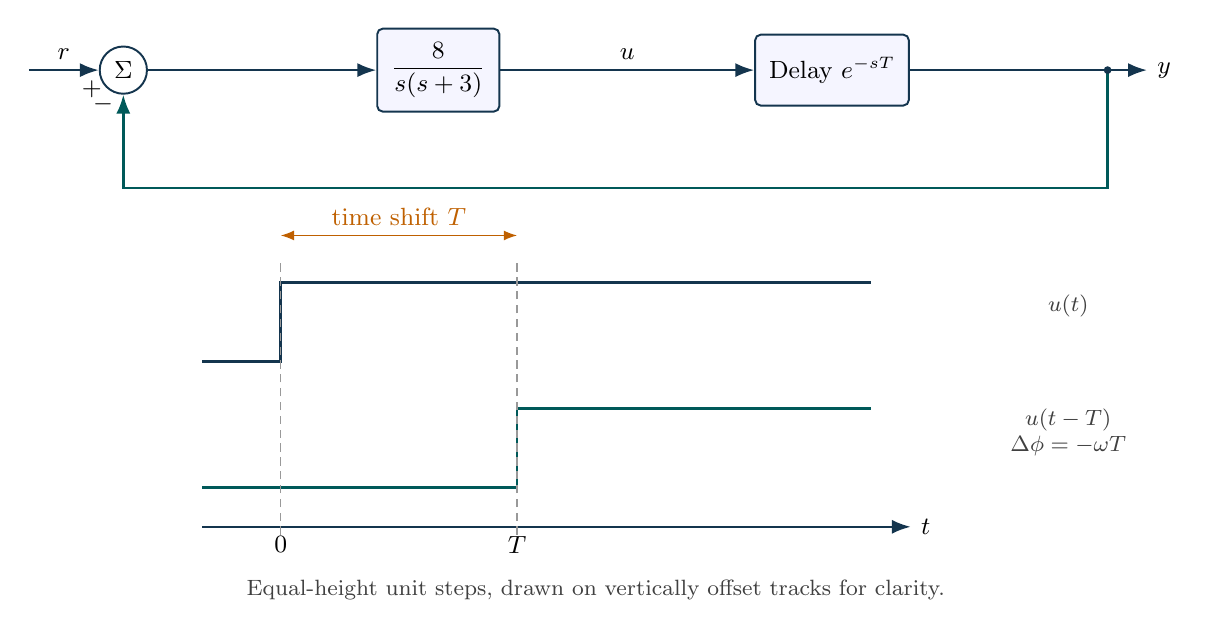
\begin{tikzpicture}[x=1cm,y=1cm,>=Latex,font=\small,
block/.style={draw=ink,fill=blue!4,rounded corners=2pt,minimum height=9mm,align=center,line width=.7pt,inner sep=5pt},
sum/.style={circle,draw=ink,fill=white,minimum size=6mm,inner sep=0pt,line width=.7pt},
sig/.style={->,draw=ink,line width=.85pt},
fb/.style={->,draw=teal!70!black,line width=.85pt},
dist/.style={->,draw=orange!75!black,line width=.85pt},
tap/.style={circle,fill=ink,inner sep=1.4pt},
note/.style={font=\footnotesize,align=center,text=black!75}]

\node[sum](e)at(1,2.1){$\Sigma$};
\node[block](g)at(5,2.1){$\dfrac{8}{s(s+3)}$};
\node[block](d)at(10,2.1){Delay $e^{-sT}$};
\draw[sig](-.2,2.1)--node[above]{$r$}node[pos=.9,below]{$+$}(e);
\draw[sig](e)--(g);\draw[sig](g)--node[above]{$u$}(d);
\draw[sig](d)--(14,2.1)node[right]{$y$};
\draw[fb](13.5,2.1)--(13.5,.6)--(1,.6)--node[pos=.9,left]{$-$}(e);
\fill[ink](13.5,2.1)circle(1.4pt);
\draw[sig](2,-3.7)--(11,-3.7)node[right]{$t$};
\draw[line width=1pt,draw=ink](2,-1.6)--(3,-1.6)--(3,-.6)--(10.5,-.6);
\draw[line width=1pt,draw=teal!70!black](2,-3.2)--(6,-3.2)--(6,-2.2)--(10.5,-2.2);
\draw[densely dashed,black!40](3,-3.8)--(3,-.35)(6,-3.8)--(6,-.35);
\node[below]at(3,-3.7){$0$};\node[below]at(6,-3.7){$T$};
\draw[<->,orange!75!black](3,0)--node[above]{time shift $T$}(6,0);
\node[note]at(13,-.9){$u(t)$};
\node[note]at(13,-2.5){$u(t-T)$\\$\Delta\phi=-\omega T$};
\node[note]at(7,-4.5){Equal-height unit steps, drawn on vertically offset tracks for clarity.};

\end{tikzpicture}
}\par{\small Constant pure delay shifts a signal in time and contributes frequency-dependent phase lag. The sketch shows ideal steps, not experimental records.}\end{center}
\begin{enumerate}
\item Write the first-order Pade approximation of $e^{-sT}$. Locate its pole and zero and explain why the right-half-plane zero does not mean the exact delay has a finite unstable zero.
\answer The approximation is $(1-Ts/2)/(1+Ts/2)$. It has pole $-2/T$ and zero $+2/T$ for $T>0$. The stable pole permits a causal rational state realization, while the zero reproduces phase lag without changing unit magnitude on the imaginary axis. The exact exponential has no finite zeros; the right-half-plane zero belongs to the rational approximation. It can generate an inverse transient absent from an exact delayed signal.
\item At the crossover of this loop, compare exact delay phase with first-order Pade phase for $T=0.3$ s. Derive the sign of the approximation error for any positive frequency.
\answer Let $x=\omega_cT/2$. Exact phase is $-2x$ radians; first-order Pade phase is $-2\arctan x$. The latter is less negative because $\arctan x<x$ for $x>0$. The phase error is $2(x-\arctan x)>0$, about $1.228^\circ$ here. Therefore this approximation slightly overestimates the remaining margin at that frequency. Increasing approximation order can reduce local error, but exact-delay conclusions should not be inferred blindly from a low-order plot.
\item Derive the first-order Padé estimate of the delay boundary at the unchanged crossover, and compare it symbolically with the exact boundary. State the direction of the error without relying on a plot.
\answer The approximated delay phase is $-2\tan^{-1}(\omega_cT/2)$. Setting it equal to $-PM_0$ gives $T_{\rm Pade}=2\tan(PM_0/2)/\omega_c$, whereas the exact result is $T_{\rm exact}=PM_0/\omega_c$. Here $0<PM_0/2<\pi/2$ and $\tan x>x$, hence $T_{\rm Pade}>T_{\rm exact}$. The first-order phase approximation is optimistic for this boundary calculation; it does not certify the exact-delay stability limit.
\end{enumerate}

\newpage
\task{4}{Sensor dynamics invalidate a previously acceptable delay budget}
A sensor lag is added after the original delay requirement was checked. Reassess the uncertain-delay interval using the modified loop.
\begin{enumerate}
\item Add sensor $1/(0.1s+1)$ to the delay-free loop. Calculate its magnitude and phase at the old crossover. Explain what must be recomputed before stating an exact new delay budget.
\answer At the old crossover the sensor magnitude is $1/\sqrt{1+0.01\omega_c^2}$ and its phase is $-\arctan(0.1\omega_c)$. The magnitude is below one, so the old crossover is no longer a unity-magnitude point. Solve $8/[\omega\sqrt{\omega^2+9}\sqrt{1+0.01\omega^2}]=1$ for the new crossover, evaluate total phase there, then divide the new margin in radians by that crossover. Subtracting only the sensor phase at the old frequency is an approximation.
\item Suppose the constant delay is uncertain in $[0.12,0.18]$ s. Find the smallest phase margin across this interval and decide whether all frozen-delay models meet a 30 degree margin. Does the result automatically cover arbitrary time-varying jitter?
\answer The margin decreases linearly with constant delay, so the worst frozen value is at 0.18 s: $\phi_{min}=\phi_m-0.18\omega_c$, approximately $31.90^\circ$. This exceeds 30 degrees, so all constant-delay models in the interval meet the stated margin criterion. Arbitrarily time-varying delay is not a linear time-invariant transfer function; frozen-delay margins alone are not a general proof of stability under jitter.
\item For the added sensor, derive the equation for the new positive crossover. Recompute the worst frozen-delay phase margin over $T\in[0.12,0.18]$ and decide whether the 30-degree requirement still holds.
\answer The crossover now satisfies $\omega^2(\omega^2+9)(1+0.01\omega^2)=64$. The left side is strictly increasing for $\omega>0$, so it has one positive solution $\omega_s$. The worst margin is $\pi/2-\tan^{-1}(\omega_s/3)-\tan^{-1}(0.1\omega_s)-0.18\omega_s$. Numerically $\omega_s\approx2.127567$ rad/s and the margin is approximately $20.7031^\circ$, below 30 degrees, so the previous guarantee fails. The executable checks compute the precise values. This remains a frozen-delay statement, not a proof for arbitrary jitter.
\end{enumerate}

\newpage
\task{5}{Trading loop speed for delay tolerance and numerical fidelity}
Reduce loop gain and compare exact-delay simulation with an approximation. Verify both the control tradeoff and the time indexing of the numerical model.
\begin{enumerate}
\item Replace numerator 8 by 4. Derive the new crossover and delay boundary and compare the control-design tradeoff.
\answer The magnitude equation becomes $\omega^4+9\omega^2-16=0$, giving $\omega_c=\sqrt{(-9+\sqrt{145})/2}$. The nominal margin is $\pi/2-\arctan(\omega_c/3)$ and the first delay boundary is that margin divided by the new crossover. It is approximately 0.95749 s, larger than for numerator 8. Reduced gain lowers bandwidth and can worsen tracking speed, so the improved delay allowance is not a free performance improvement.
\item An exact delayed plant response is zero before delay T when initial conditions are zero. Explain why a finite-order Pade simulation may respond immediately. Describe a reproducible numerical check for a delay-buffer simulation.
\answer A rational Pade model replaces the time shift with finite-dimensional dynamics, so its impulse response is generally nonzero before T; it does not implement a literal waiting interval. For a buffer with sample interval $h$ and integer delay $N=T/h$, verify that the driven plant receives zero input for its first N intervals and then receives the appropriately indexed past command. Repeat with smaller h while preserving the intended delay. This checks indexing and convergence of the numerical scheme, not physical equipment.
\item Represent a 0.605 s delay using a 0.01 s step and integer-sample rounding. Bound the resulting delay error and its phase error at the new crossover. Propose a grid that represents the stated delay exactly.
\answer The delay lies halfway between 60 and 61 samples. Rounding introduces absolute error 0.005 s, with phase error at crossover bounded by $0.005\omega_{c,4}$ radians. This error can matter when a design uses almost all its phase reserve. A step of 0.005 s represents 0.605 s as exactly 121 intervals. Grid refinement should compare trajectories and metrics as well as checking zero response before the intended onset; a visually smooth Padé response is not an indexing test.
\end{enumerate}

\end{document}
